% ModelEvaluation

\chapter{Évaluation des modèles} % Main chapter title

\label{ModelEvaluation} % For referencing the chapter elsewhere, use \ref{ModelEvaluation} 

%----------------------------------------------------------------------------------------

Dans les chapitres "Réseaux de neurones utilisés" (\ref{UsedModels}) et "Résultats" (\ref{Results}), nous allons aborder différentes métriques pour évaluer nos modèles. Afin de comprendre ce qu'elles signifient et comment elles ont été calculées, nous allons les détailler dans les sections suivantes.

\section{Intersection sur union}
\label{sec:iou}

L'intersection sur union (\acrfull{iou} en anglais) \cite{subramanyam_iouintersection_2021} est une métrique très utile pour évaluer la précision d'une prédiction par rapport à sa réalité. Celle-ci s'applique notamment aux tâches de détection et de segmentation.

Nous pouvons expliquer ce concept intuitivement avec la figure \ref{fig:iou_prediction_and_ground_truth}, où le carré rouge correspond à la prédiction réalisée, tandis que le carré vert correspond à la délimitation du panneau "STOP". 

\begin{figure}[hbt!]
    \centering
    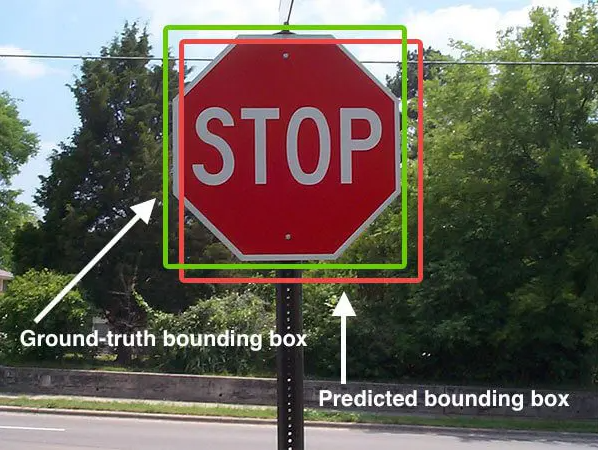
\includegraphics[scale=0.5]{Figures/model_evaluation/iou_prediction_and_ground_truth.png}
    \caption{Représentation de la formule de l'intersection sur union \cite{noauthor_jaccard_2023}.}
    \label{fig:iou_prediction_and_ground_truth}
\end{figure}

Comme son nom l'indique, l'\acrshort{iou} est définie par l'intersection, la zone qui se chevauche entre la boîte prédite et celle de référence, sur l'union, la zone couverte par les deux boîtes, comme nous pouvons le voir sur la figure \ref{fig:iou_formula}.

\begin{figure}[hbt!]
    \centering
    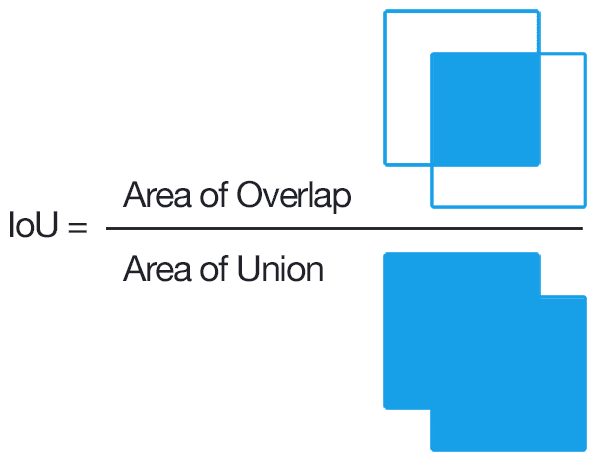
\includegraphics[scale=0.5]{Figures/model_evaluation/iou_formula.png}
    \caption{Représentation de la formule de l'intersection sur union \cite{noauthor_jaccard_2023}.}
    \label{fig:iou_formula}
\end{figure}

\break

Celle-ci est formellement décrite par la formule :

\[IoU=\frac{Aire \: de \: chevauchement}{Aire \: d'union}\]

Le résultat de ce cette opération est un nombre entre $0$ et $1$, où $0$ correspond à aucun chevauchement, et $1$ indique un chevauchement parfait.

Il peut être utilisé comme seuil pour déterminer si une prédiction est juste ou non. Dans notre travail, nous considérons une détection comme correcte si celle obtiens au moins $0.5$ de \acrshort{iou}. Cette valeur est très couramment utilisée, car elle offre un bon compromis entre la précision et la tolérance, de plus des compétitions comme The PASCAL Visual Object Classes (VOC) Challenge \cite{everingham_pascal_2010} en ont fait le seuil à adopter. Cependant, il est possible de l'adapter en fonction du projet.

\section{Matrice de confusion}

Une matrice de confusion est un outil qui permet de visualiser les performances d'un algorithme, notamment dans le domaine de l'apprentissage supervisé \cite{karimi_confusion_2021}.

Bien que nous ne l'utilisons pas directement dans nos résultats, nous utilisons plusieurs métriques issues de cette dernière que nous détaillerons dans leurs sous-sections respectives.

Celle-ci peut-être représentée sous la forme d'une matrice à deux dimensions comme sur la table \ref{tab:confusion_matrix}, où dans notre cas, la première correspond aux éléments réels, et la seconde aux prédictions de nos modèles.

\begin{table}[!ht]
    \caption{Représentation d'une matrice de confusion}
    \label{tab:confusion_matrix}
    \centering
    \begin{tabular}{|c|c|c|c|  }
        \hhline{----}
        \multicolumn{2}{|c|}{} & \multicolumn{2}{c|}{\cellcolor{gray!50} Prédit}\\
        \hhline{~~--}
        \multicolumn{2}{|c|}{} & \cellcolor{gray!25}Positif & \cellcolor{gray!25}Négatif\\
        \hhline{----}
        \cellcolor{gray!50} & \cellcolor{gray!25}Positif & Vrai positif & Faux négatif\\
        \arrayrulecolor{gray!50}
        \cline{1-1}
        \arrayrulecolor{black}
        \hhline{~---}
        \multirow{-2}{*}{\cellcolor{gray!50} Réel} & \cellcolor{gray!25}Négatif & Faux positif & Vrai négatif\\
        \hline
    \end{tabular}
\end{table}

\break

\subsection{Vrais / Faux - positifs / négatifs}

Lorsqu'une prédiction est réalisée, celle-ci va être placée dans la matrice de confusion. 
Comme nous pouvons l'observer sur la table \ref{tab:confusion_matrix}, cette dernière est composée de quatre catégories :\\

\begin{itemize}
    \item \textbf{Vrai positif} : La prédiction est correcte.
    \item \textbf{Faux positif} : La prédiction est fausse.
    \item \textbf{Faux négatif} : Un élément réel qui n'a pas été prédit.
    \item \textbf{Vrai négatif} : Ne s'applique pas dans notre cas. Cependant, il s'agirait d'aucune détection où il n'y a rien à détecter. Or, dans les problèmes de détection d'objets, il y a un grand nombre de zones sur une image qui ne doivent pas être détectées, et les vrais négatifs correspondraient à toutes ces zones correctement non détectées. Ainsi, nous n'utiliserons aucune métrique la nécessitant, et la valeur de ce cas sera nulle.\\
\end{itemize}

Comme nous venons de le voir, les détections à elles seules ne suffisent pas à remplir la matrice de confusion. Il nous faut également les éléments réels de l'image que notre modèle tente de détecter. Ceux-ci nous permettront d'identifier si une détection est correcte ou non, en utilisant par exemple l'\acrshort{iou}, et de compléter notre table lorsque toutes les détections auront été traitées, s'il reste des éléments réels qui n'ont pas été détectés.\\

À ce stade, à l'aide de notre matrice de confusion, nous pouvons déjà constater la capacité d'un modèle à réaliser des détections correctes, et observer si celui-ci a une tendance (ou non) à prédire trop de faux positifs, ou au contraire à réaliser trop des faux négatifs. De telles informations se révèlent très utiles pour affiner certains seuils utilisés comme le score de confidence minimum pour prendre en compte une détection, mais aussi comment les résultats se comportent avec un l'\acrshort{iou} plus élevé. Ceux-ci devront être adaptés en fonction des applications et des tolérances.

À partir de ces données, nous allons pouvoir calculer une partie des métriques que nous utilisons et analysons dans le chapitre résultats (\ref{Results}), afin de mieux comprendre le comportement du modèle utilisé.

\subsection{Précision}

La précision correspond à la proportion d'éléments corrects parmi tous ceux prédits par le modèle. Elle est décrite par la formule suivante :

\[pr\acute{e}cision = \frac{vrais \: positifs}{vrais \: positifs + faux \: positifs}\]

Celle-ci permet donc d'évaluer la capacité du modèle à réaliser des prédictions correctes. Cependant, il est nécessaire de l'associer à d'autres métriques comme le rappel. En effet, en utilisant uniquement les vrais positifs et les faux positifs, la précision n'est pas sensible aux faux négatifs. Ainsi, il est très probable d'obtenir un résultat de $100\%$ en ne sélectionnant que quelques éléments détectés pour lesquels le modèle possède un score de confiance très élevé. En contrepartie, il est très probable que ce dernier n'ait pas détecté tous les éléments réels, mais cela n'apparaît pas dans cette métrique.

\subsection{Rappel}

Le rappel correspond à la proportion d'éléments prédits correctement parmi tous les éléments réels à prédire. Il est décrit par la formule suivante :

\[rappel = \frac{vrais \: positifs}{vrais \: positifs + faux \: n\acute{e}gatifs}\]

Celui-ci permet d'évaluer la capacité du modèle à détecter les éléments attendus. Tout comme pour la précision, il est nécessaire d'associer le rappel à d'autres métriques comme à cette dernière par exemple. Effectivement, à présent nous utilisons les vrais positifs et faux négatifs, rendant le rappel insensible aux faux positifs. En acceptant toutes les prédictions de notre modèle, même celles pour lesquelles le score de confiance du modèle est nul, nous pourrions alors obtenir un score de rappel très élevé au détriment de la précision.

\subsection{Courbe précision rappel}

La courbe précision rappel permet, comme son nom l'indique, de visualiser l'évolution de la précision en fonction du rappel pour le modèle évalué. Celle-ci est tracée en diminuant progressivement le seuil du score de confiance des prédictions réalisées. De plus, dans le cadre de la détection d'objets, l'\acrshort{iou} est également utilisé afin définir si une prédiction est correcte ou non.\\

La courbe parfaite, comme illustrée par la figure \ref{fig:perfect_precision_recall_curve}, est une courbe pour laquelle peut importe le rappel, la précision reste à $1$. Cela signifie que le modèle évalué est capable de détecter tous les éléments réels sans faire d'erreurs.

\begin{figure}[hbt!]
    \centering
    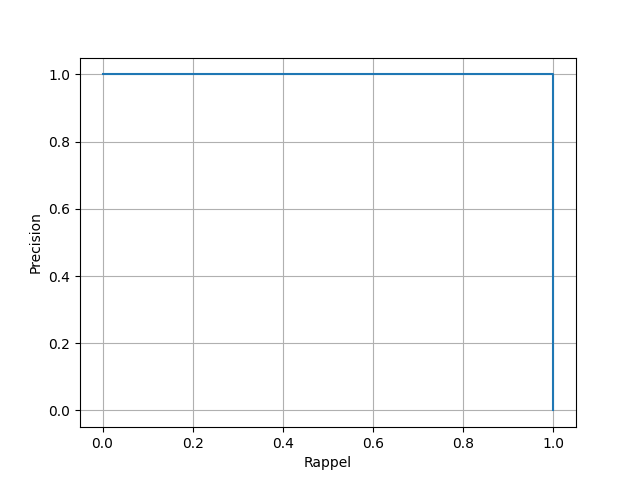
\includegraphics[scale=0.7]{Figures/model_evaluation/perfect_precision_recall_curve.png}
    \caption{Courbe précision rappel parfaite}
    \label{fig:perfect_precision_recall_curve}
\end{figure}

\break

Ainsi, lorsqu'une courbe adopte un tracé haut et vers la droite, qui tend vers cette courbe idéale, celle-ci nous indique que le modèle performe bien. Il possède alors une précision élevée pour un rappel élevé, et il détecte correctement la plupart des éléments tout en minimisant les faux positifs.

Inversement, une courbe basse et vers la gauche indique que le modèle possède de piètres performances.

\subsection{Average precision et mean average precision}

L'\acrfull{ap} (précision moyenne en français) correspond à l'aire sous la courbe précision rappel \cite{padilla_rafaelpadillaobject-detection-metrics_2024}. Celle-ci permet d'évaluer les performances d'un modèle sans fixer de seuil pour le score de confiance, et par conséquent, d'obtenir une mesure unique combinant à la fois la précision et le rappel pour un seuil d'\acrshort{iou} donné.

Cette dernière est calculée à l'aide de la formule suivante :

\[\acrfull{ap} = \int_{0}^{1} p(r)dr\]

Où la fonction $p(r)$ correspond à la courbe précision rappel précédemment calculée.\\

Cette mesure est liée à une classe et doit être recalculée pour toutes les classes prédites par le modèle. À partir des différents \acrshort{ap}, il est alors possible de calculer la \acrfull{map} (la moyenne de la précision moyenne) à l'aide de la formule :

\[\acrfull{map}=\frac{1}{k}\sum_{i=0}^{k}AP_i\]

Où $k$ correspond au nombre de classes, et $AP_i$ l'\acrshort{ap} pour la classe $i$.

Dans notre cas, comme nous ne travaillons qu'avec une classe, l'\acrshort{ap} et la \acrshort{map} sont identiques.

Comme souligné plus tôt, le résultat obtenu est celui pour un \acrshort{iou} donné. Nous avons également déjà abordé dans sa section (\ref{sec:iou}) que celui-ci est généralement égal à $0.5$. Nous pouvons donc faire varier cette valeur pour observer l'évolution de l'\acrshort{ap} à différents seuils. Cependant, il reste complexe et arbitraire de choisir d'autres valeurs de seuil. Ainsi, nous avons décidé d'utiliser la métrique principale d'évaluation utilisée par \acrshort{coco}, c'est-à-dire l'\acrshort{ap} à un \acrshort{iou} de $.5:.05:.95$ \cite{noauthor_coco_nodate}. Cela signifie que nous calculons l'\acrshort{ap} pour les \acrshort{iou} en commençant à $0.5$ jusqu'à $0.95$ avec un pas de $0.05$, puis nous réalisons la moyenne de tous les \acrshort{ap} obtenus.

Cette fois-ci non seulement nous obtenons un résultat qui n'est pas sensible au seuil de confiance, mais nous obtenons également une valeur qui prend en compte la capacité du modèle à effectuer des détections de plus en plus précises.

\subsection{Score F1}

La dernière métrique utilisée est le score F1. Il s'agit de la moyenne harmonique de la précision et du rappel, nous permettant d'évaluer la performance du modèle. Il est décrit par la formule suivante :

\[score \: F_1 = 2 \cdot \frac{pr\acute{e}cision \cdot rappel}{pr\acute{e}cision + rappel} = \frac{2 \cdot vrais \: positifs}{2 \cdot vrais \: positifs + faux \: positifs + faux \: n\acute{e}gatifs}\]

Ce rapport s'avère précieux et complémentaire pour observer la qualité des prédictions réalisées dans un contexte où la précision et le rappel sont les deux très importants. Un score de $1$ signifierait que toutes les détections traitées étaient correctes et qu'elles couvraient l'ensemble des éléments à détecter. Un score F1 proche de $1$ indique des performances élevées, au contraire d'un résultat autour de $0.5$ indiquant que le modèle à des difficultés avec la précision, le rappel, ou les deux.


%----------------------------------------------------------------------------------------
